\documentclass{article}
\usepackage{tikz}
\usetikzlibrary{arrows, shapes, positioning}
%\tikzstyle{nodeobserved} = [circle, minimum size = 10mm, thick, draw =black!80]
\usetikzlibrary{external}
\tikzexternalize


\begin{document}

\begin{figure}
    \centering
    \tikzsetnextfilename{dag-fire0}
        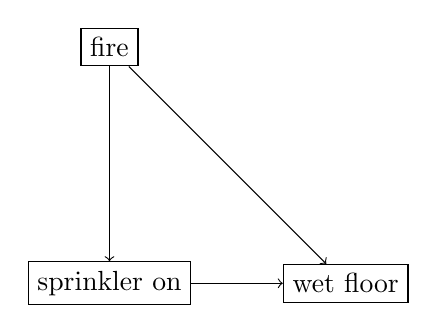
\begin{tikzpicture}
          % Nodes
          \node[draw] (z) at (0, 3) {fire};
          \node[draw] (t) at (0, 0) {sprinkler on};
          \node[draw] (y) at (3, 0) {wet floor};

          % Edges
          \draw[->] (z) -- (t);
          \draw[->] (z) -- (y);
          \draw[->] (t) -- (y);

        \end{tikzpicture}
\end{figure}

\begin{figure}
    \centering
    \tikzsetnextfilename{dag-floor1}

    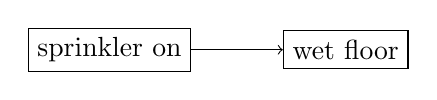
\begin{tikzpicture}
      % Nodes
      \node[draw] (t) at (0, 0) {sprinkler on};
      \node[draw] (y) at (3, 0) {wet floor};

      % Edges
      \draw[->] (t) -- (y);

    \end{tikzpicture}
        
\end{figure}

\begin{figure}
    \centering
    \tikzsetnextfilename{dag-floor2}
        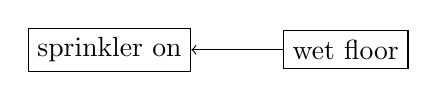
\begin{tikzpicture}
          % Nodes
          \node[draw] (t) at (0, 0) {sprinkler on};
          \node[draw] (y) at (3, 0) {wet floor};

          % Edges
          \draw[->] (y) -- (t);
        \end{tikzpicture}
        
\end{figure}


\begin{figure}
    \centering
    \tikzsetnextfilename{dag-fire1}
    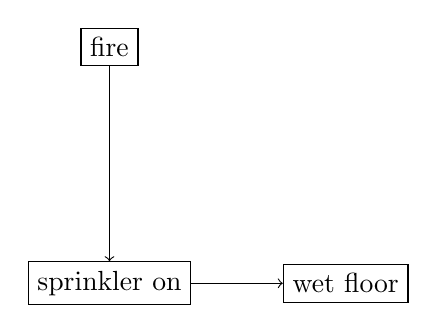
\begin{tikzpicture}
      % Nodes
      \node[draw] (z) at (0, 3) {fire};
      \node[draw] (t) at (0, 0) {sprinkler on};
      \node[draw] (y) at (3, 0) {wet floor};

      % Edges
      \draw[->] (z) -- (t);
      \draw[->] (t) -- (y);

    \end{tikzpicture}
\end{figure}

\begin{figure}
    \centering

    \tikzsetnextfilename{dag-fire2}
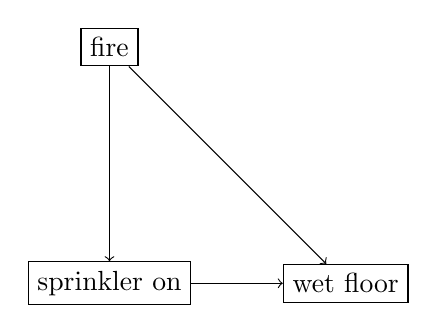
\begin{tikzpicture}
  % Nodes
  \node[draw] (z) at (0, 3) {fire};
  \node[draw] (t) at (0, 0) {sprinkler on};
  \node[draw] (y) at (3, 0) {wet floor};

  % Edges
  \draw[->] (z) -- (t);
  \draw[->] (z) -- (y);
  \draw[->] (t) -- (y);

\end{tikzpicture}

\end{figure}

\begin{figure}
    \centering

    \tikzsetnextfilename{dag-fire3}
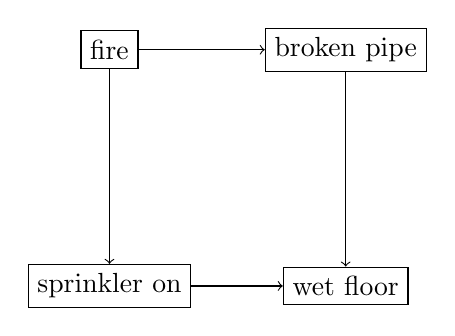
\begin{tikzpicture}
  % Nodes
  \node[draw] (z) at (0, 3) {fire};
  \node[draw] (m) at (3, 3) {broken pipe};
  \node[draw] (t) at (0, 0) {sprinkler on};
  \node[draw] (y) at (3, 0) {wet floor};

  % Edges
  \draw[->] (z) -- (t);
  \draw[->] (z) -- (m);
  \draw[->] (m) -- (y);
  \draw[->] (t) -- (y);

\end{tikzpicture}

\end{figure}

\begin{figure}
    \centering

    \tikzsetnextfilename{dag-nonparametric}
\begin{tikzpicture}
  % Nodes
  \node (z) at (0, 1) {$X$};
  \node (t) at (-1, 0) {$T$};
  \node (y) at (0, 0) {$Y$};

  % Edges
  \draw[->] (z) -- (y);
  \draw[->] (t) -- (y);

\end{tikzpicture}

\end{figure}

\begin{figure}
    \centering

    \tikzsetnextfilename{dag-delivery}
  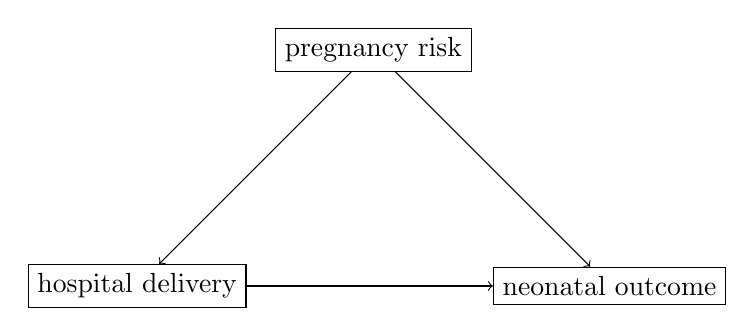
\begin{tikzpicture}
    % Nodes
    \node[draw] (z) at (0, 3) {pregnancy risk};
    \node[draw] (t) at (-3, 0) {hospital delivery};
    \node[draw] (y) at (3, 0) {neonatal outcome};

    % Edges
    \draw[->] (z) -- (t);
    \draw[->] (z) -- (y);
    \draw[->] (t) -- (y);

  \end{tikzpicture}

\end{figure}

\begin{figure}
    \centering

    \tikzsetnextfilename{dag-delivery-int}
  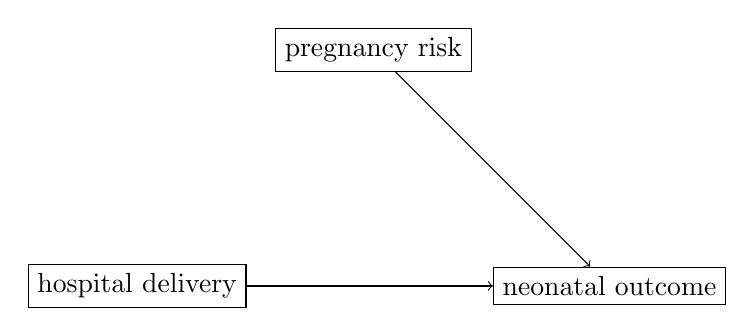
\begin{tikzpicture}
    % Nodes
    \node[draw] (z) at (0, 3) {pregnancy risk};
    \node[draw] (t) at (-3, 0) {hospital delivery};
    \node[draw] (y) at (3, 0) {neonatal outcome};

    % Edges
    \draw[->] (z) -- (y);
    \draw[->] (t) -- (y);

  \end{tikzpicture}

\end{figure}



\begin{figure}
    \centering

    \tikzsetnextfilename{dag-hernia}
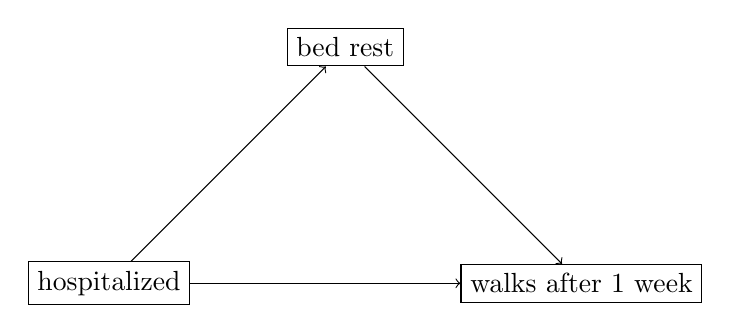
\begin{tikzpicture}
  % Nodes
  \node[draw] (z) at (0, 3) {bed rest};
  \node[draw] (t) at (-3, 0) {hospitalized};
  \node[draw] (y) at (3, 0) {walks after 1 week};

  % Edges
  \draw[->] (t) -- (z);
  \draw[->] (z) -- (y);
  \draw[->] (t) -- (y);

\end{tikzpicture}

\end{figure}

\begin{figure}
    \centering

    \tikzsetnextfilename{dag-fork}
        \begin{tikzpicture}
          % Nodes
          \node (z) at (0, 1) {$Z$};
          \node (x) at (-1, 0) {$X$};
          \node (y) at (1, 0) {$Y$};

          % Edges
          \draw[->] (z) -- (x);
          \draw[->] (z) -- (y);

        \end{tikzpicture}

\end{figure}

\begin{figure}
    \centering

    \tikzsetnextfilename{dag-dag1x}
        \begin{tikzpicture}
          % Nodes
          \node (z) at (0, 1) {$Z$};
          \node (x) at (-1, 0) {$X$};
          \node (y) at (1, 0) {$Y$};

          % Edges
          \draw[->] (z) -- (x);
          \draw[->] (z) -- (y);
          \draw[->] (x) -- (y);

        \end{tikzpicture}

\end{figure}

\begin{figure}
    \centering

    \tikzsetnextfilename{dag-chain}
        \begin{tikzpicture}
          % Nodes
          \node (m) at (0, 1) {$M$};
          \node (x) at (-1, 0) {$X$};
          \node (y) at (1, 0) {$Y$};

          % Edges
          \draw[->] (x) -- (m);
          \draw[->] (m) -- (y);

        \end{tikzpicture}

\end{figure}

\begin{figure}
    \centering

    \tikzsetnextfilename{dag-collider}
        \begin{tikzpicture}

          % Nodes
          \node (z) at (0, 1) {$Z$};
          \node (x) at (-1, 0) {$X$};
          \node (y) at (1, 0) {$Y$};

          % Edges
          \draw[->] (x) -- (z);
          \draw[->] (y) -- (z);

        \end{tikzpicture}

\end{figure}

\begin{figure}
    \centering

    \tikzsetnextfilename{dag-obs}
        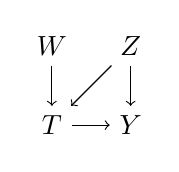
\begin{tikzpicture}
            % Nodes
            \node (w) at (0, 1) {$W$};
            \node (z) at (1, 1) {$Z$};
            \node (t) at (0, 0) {$T$};
            \node (y) at (1, 0) {$Y$};
            
            % Edges
            \draw[->] (w) -- (t);
            \draw[->] (z) -- (t);
            \draw[->] (z) -- (y);
            \draw[->] (t) -- (y);
        \end{tikzpicture}
        
    \end{figure}

\begin{figure}
    \centering

    \tikzsetnextfilename{dag-intervened}
    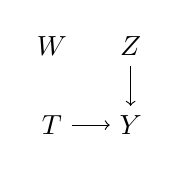
\begin{tikzpicture}
        \node (w) at (0, 1) {$W$};
        \node (z) at (1, 1) {$Z$};
        \node (t) at (0, 0) {$T$};
        \node (y) at (1, 0) {$Y$};
        
        \draw[->] (z) -- (y);
        \draw[->] (t) -- (y);
    \end{tikzpicture}
    
\end{figure}

\begin{figure}
    \begin{center}
    \tikzsetnextfilename{dag1-obs}
        \begin{tikzpicture}
            \node (z) at (0, 1) {$Z$};
            \node (t) at (-1, 0) {$T$};
            \node (y) at (1, 0) {$Y$};
            
            \draw[->] (z) -- (y);
            \draw[->] (z) -- (t);
            \draw[->] (t) -- (y);
        \end{tikzpicture}
    \end{center}
\end{figure}

\begin{figure}
    \begin{center}
    \tikzsetnextfilename{dag1-intervened}
        \begin{tikzpicture}
            \node (z) at (0, 1) {$Z$};
            \node (t) at (-1, 0) {$T$};
            \node (y) at (1, 0) {$Y$};
            
            \draw[->] (z) -- (y);
            \draw[->] (t) -- (y);
        \end{tikzpicture}
    \end{center}
\end{figure}


\begin{figure}
    \begin{center}
    \tikzsetnextfilename{path1}
        \begin{tikzpicture}
            \node (x) at (-3, 0) {$x$};
            \node (r) at (-2, 0) {$r$};
            \node (s) at (-1, 0) {$s$};
            \node (t) at (0, -1) {$t$};
            \node (u) at (1, 0) {$u$};
            \node (v) at (2, 1) {$v$};
            \node (y) at (3, 0) {$y$};
            
            \draw[->] (x) -- (r);
            \draw[->] (r) -- (s);
            \draw[->] (s) -- (t);
            \draw[->] (v) -- (u);
            \draw[->] (u) -- (t);
            \draw[->] (v) -- (y);
        \end{tikzpicture}
    \end{center}
\end{figure}


\begin{figure}
    \begin{center}
    \tikzsetnextfilename{path1z}
        \begin{tikzpicture}
            \node (x) at (-3, 0) {$x$};
            \node[draw,circle] (r) at (-2, 0) {$r$};
            \node (s) at (-1, 0) {$s$};
            \node[draw,circle] (t) at (0, -1) {$t$};
            \node (u) at (1, 0) {$u$};
            \node (v) at (2, 1) {$v$};
            \node (y) at (3, 0) {$y$};
            

            \draw[->] (x) -- (r);
            \draw[->] (r) -- (s);
            \draw[->] (s) -- (t);
            \draw[->] (v) -- (u);
            \draw[->] (u) -- (t);
            \draw[->] (v) -- (y);
        \end{tikzpicture}
    \end{center}
\end{figure}

\begin{figure}
    \begin{center}
        \tikzsetnextfilename{house}
        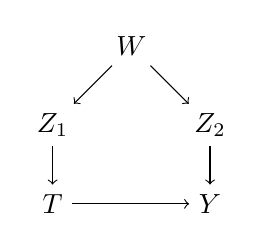
\begin{tikzpicture}
            \node (w) at (1, 2) {$W$};
            \node (z1) at (0, 1) {$Z_1$};
            \node (z2) at (2, 1) {$Z_2$};
            \node (t) at (0, 0) {$T$};
            \node (y) at (2, 0) {$Y$};

            \draw[->] (w) -- (z1);
            \draw[->] (w) -- (z2);
            \draw[->] (z1) -- (t);
            \draw[->] (z2) -- (y);
            \draw[->] (t) -- (y);
        \end{tikzpicture}
        
    \end{center}
    
\end{figure}


\end{document}
